\documentclass{article}

\usepackage{graphicx}
\usepackage{tikz}
\usepackage{tikzsymbols}
\usetikzlibrary{calc,patterns,shapes.geometric}
\pagestyle{empty}
\usepackage[margin=0pt]{geometry}
\geometry{papersize={14in,12in}}

\def\centerarc[#1](#2)(#3:#4:#5){\draw[#1] ($(#2)+({#5*cos(#3)},{#5*sin(#3)})$) arc (#3:#4:#5);}

\begin{document}
	\begin{figure}
		\centering
		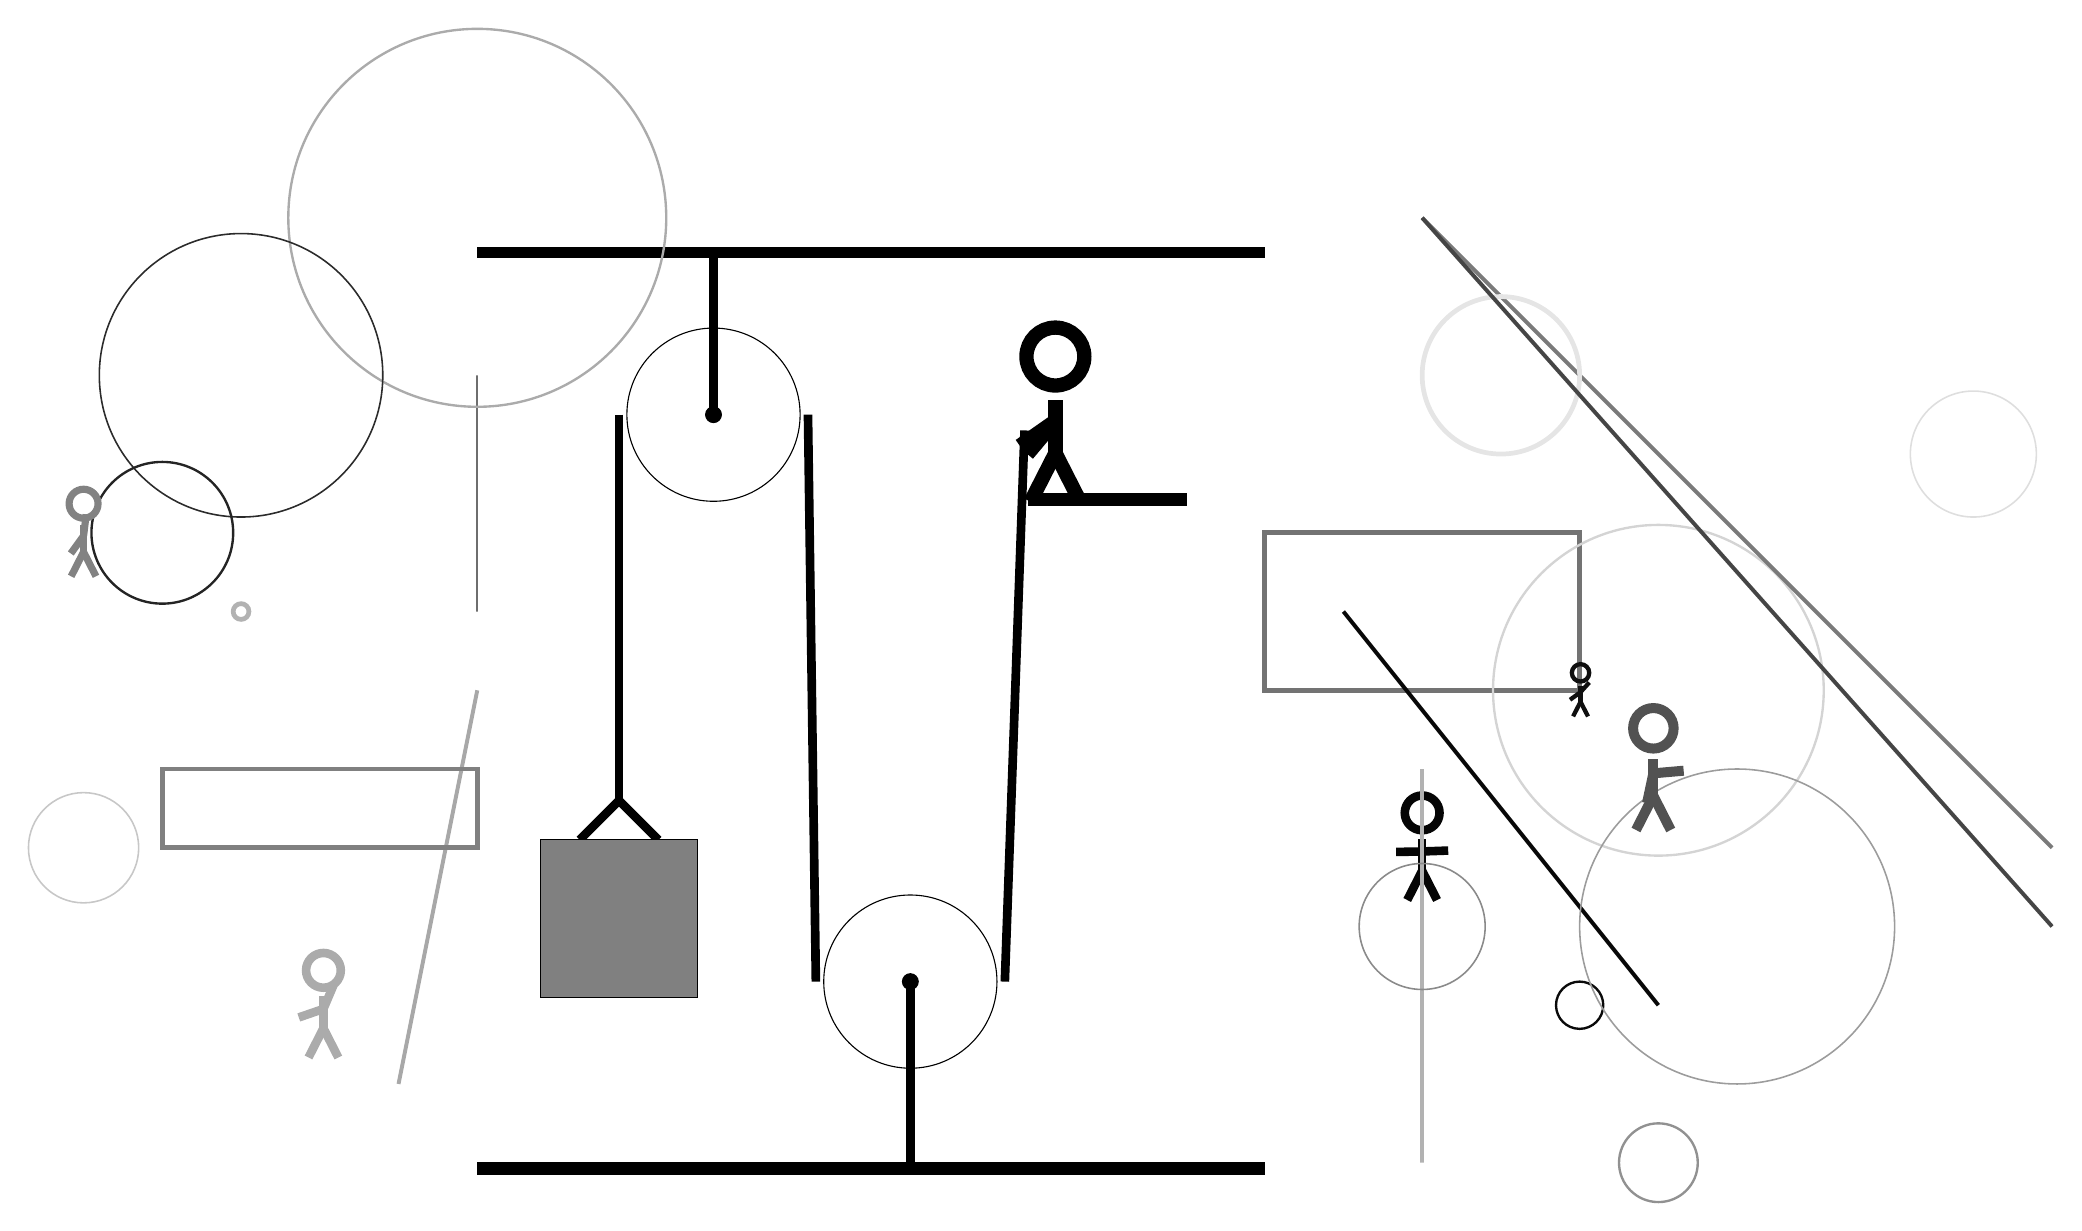
\begin{tikzpicture}
			%%%%% START %%%%%
			
			\draw[fill=black] (-2, 11.5) rectangle (8, 11.625);
			
			\draw (3.5, 2.3) circle (1.1);
			\draw[fill=black] (3.5, 2.3) circle (0.1);
			\draw[line width=1.1mm] (3.5, 2.3) -- (3.5, 0);
			
			\draw (1, 9.5) circle (1.1);
			\draw[fill=black] (1, 9.5) circle (0.1);
			\draw[line width=1.1mm] (1, 11.5) -- (1, 9.5);
			
			\draw [line width=0.6mm, color=black!30](-5, 7) circle (0.1);
			
			\draw[line width=0.2mm, color=black!57] (-2, 7) rectangle (-2, 10);
			\draw [line width=0.2mm, color=black!13](17, 9) circle (0.8);
			\draw[line width=0.6mm, color=black!55] (8, 6) rectangle (12, 8);
			\node[line width=0.6mm, color=black!33] at (-4, 2) {\Strichmaxerl[6][19][67]};
			\draw [line width=0.3mm, color=black!17](13, 6) circle (2.1);
			\node[line width=0.5mm, color=black!98] at (10, 4) {\Strichmaxerl[6][1][2]};
			\draw [line width=0.3mm, color=black!96](12, 2) circle (0.3);
			\draw[line width=0.5mm, color=black!97](9, 7) -- (13, 2);
			\draw [line width=0.3mm, color=black!33](-2, 12) circle (2.4);
			\draw [line width=0.2mm, color=black!39](14, 3) circle (2.0);
			\draw[line width=0.5mm, color=black!52](10, 12) -- (18, 4);
			\draw [line width=0.2mm, color=black!83](-5, 10) circle (1.8);
			
			\node[line width=0.2mm, color=black!94] at (12, 6) {\Strichmaxerl[3][36][48]};
			\draw [line width=0.6mm, color=black!10](11, 10) circle (1.0);
			\draw[line width=0.5mm, color=black!34](-3, 1) -- (-2, 6);
			
			\draw [line width=0.3mm, color=black!86](-6, 8) circle (0.9);
			\draw[line width=0.6mm, color=black!50] (-2, 5) rectangle (-6, 4);
			\node[line width=0.4mm, color=black!68] at (13, 5) {\Strichmaxerl[7][78][5]};
			\draw[line width=0.5mm, color=black!30] (10, 5) rectangle (10, 0);
			\draw [line width=0.2mm, color=black!46](10, 3) circle (0.8);
			\node[line width=0.5mm, color=black!49] at (-7, 8) {\Strichmaxerl[5][54][83]};
			\draw [line width=0.3mm, color=black!43](13, 0) circle (0.5);
			\draw[line width=0.5mm, color=black!73](10, 12) -- (18, 3);
			\draw [line width=0.2mm, color=black!22](-7, 4) circle (0.7);
			
			\draw[line width=1.1mm](-0.7, 4.1) --  (-0.2, 4.6) -- (0.3, 4.1);
			\draw[fill=black!50] (-1.2, 4.1) rectangle (0.8, 2.1);
			
			\draw[line width=1.1mm](-0.2, 9.5) -- (-0.2, 4.6);
			\centerarc[line width=1.1mm](1, 9.5)(180:0:1.2000000000000002)
			\draw[line width=1.1mm](2.2, 9.5) -- (2.3, 2.3);
			\centerarc[line width=1.1mm](3.5, 2.3)(180:360:1.2000000000000002)
			\draw[line width=1.1mm](4.7, 2.3) -- (4.95, 9.3);
			
			\node at (5.3, 9.5) {\Strichmaxerl[10][35][-130]};
			\draw[fill=black] (5, 8.5) rectangle (7, 8.35);
			
			\draw[fill=black] (-2, 0) rectangle (8, -0.15);
			
			%%%%% END %%%%%
		\end{tikzpicture}
	\end{figure}	
\end{document}